\subsection*{Computation, Computer Vision and AI}
%--------------------------------------------------------------------------------------------------
\begin{frame}[t]
    \frametitle{Computation, Computer Vision and AI}
    \framesubtitle{Computation}
    \begin{columns}[t]
        \column{.5\textwidth}
        \begin{center}
            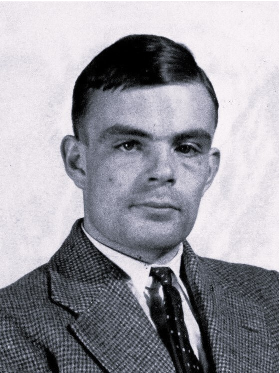
\includegraphics[width=.6\linewidth]{fig/intro/comp_cv_ai/img/turing.pdf}\\
        \end{center}
        {\small \emph{Alan Turing} forefather of current computer science.}
        \column{.5\textwidth}
        Better known as \emph{Computer Science}.\\\vspace{10pt}
        \pause
        Study of:
        \begin{itemize}
            \item Algorithms.
            \item Data structures.
            \item Design of hardware and software.
        \end{itemize}
    \end{columns}
\end{frame}
%--------------------------------------------------------------------------------------------------
\begin{frame}[t]
    \frametitle{Computation, Computer Vision and AI}
    \framesubtitle{Computer Vision}
    \begin{columns}[t]
        \column{0.5\textwidth}
            Replication of human vision capabilities.\\\vspace{10pt}\pause
            Three fundamental tasks\cite{malik2016three}:
            \begin{itemize}
                \item Recognition.
                \item Reconstruction.
                \item Reorganization.
            \end{itemize}
        \column{0.5\textwidth}
            \begin{center}
                %\begin{figure}[H]
    \scalebox{.65}{%
    \begin{tikzpicture}[]
        %% CNN branch
        \node(recon) at (3, 3.3541){Recognition};
        \node(reconst) at (0, 0) {Reconstruction};
        \node(reorg) at (6, 0) {Reorganization};

        \draw[-Stealth] ([xshift=-6pt] reconst.north) -- node {} ([xshift=-6pt] recon.south);
        \draw[-Stealth] ([xshift=-2pt] recon.south) -- node {} ([xshift=-2pt] reconst.north);

        \draw[-Stealth] ([xshift=2pt] recon.south) -- node {} ([xshift=2pt] reorg.north);
        \draw[-Stealth] ([xshift=6pt] reorg.north) -- node {} ([xshift=6pt] recon.south);

        \draw[-Stealth] ([yshift=2pt] reconst.east) -- node {} ([yshift=2pt] reorg.west);
        \draw[-Stealth] ([yshift=-2pt] reorg.west) -- node {} ([yshift=-2pt] reconst.east);        
    
    \end{tikzpicture}
    }
    %\caption{\cite{malik2016three}}
    %\label{fig:malik_rs}
%\end{figure}
            \end{center}
    \end{columns}
\end{frame}
%--------------------------------------------------------------------------------------------------
\begin{frame}[t]
    \frametitle{Computation, Computer Vision and AI}
    \framesubtitle{Artificial Intelligence}
    \begin{columns}[t]
        \begin{column}{0.5\textwidth}
        Systems capable of performing tasks requiring human intelligence 
        \cite{mccarthy2007artificial}.\\\vspace{10pt}\pause

        Subfields:
            \begin{itemize}
                \item Machine Learning \emph{(ML)} \& Deep Learning (\emph{DL}).
                \item Computer Vision(\emph{CV}).
                \item Natural Language Processing (\emph{NLP}).
                \item Robotics.
            \end{itemize}
        \end{column}
        \begin{column}{0.5\textwidth}
            \begin{center}
                \scalebox{.65}{%
    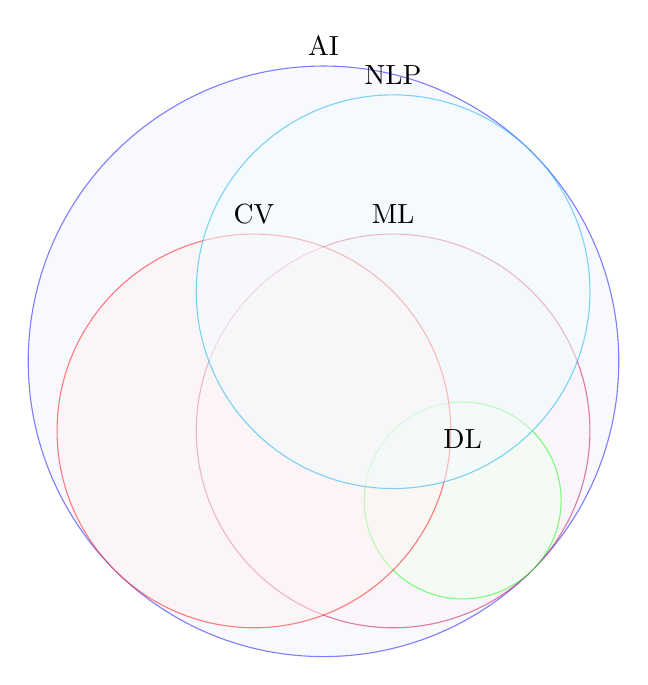
\begin{tikzpicture}[] 
            %% Anchors
            \node[circle, opacity=0.5, draw=blue, fill=blue!5, minimum size=7.5cm] 
                (aiabig) at (0, 0) {};
            \node[circle, opacity=0.5, draw=purple, fill=purple!5, minimum size= 5cm]
                (ml) at (0.8838834764831843, -0.8838834764831843) {};
            \node [circle, opacity=0.5, draw=green, fill=green!5, minimum size=2.5cm]
                (dl) at (1.7677669529663687, -1.7677669529663687) {};
            \node[circle,  opacity=0.5, draw=red, fill=red!5, minimum size=5cm]
                (cv) at (-0.8838834764831843, -0.8838834764831843) {};
            \node[circle,  opacity=0.5, draw=cyan, fill=cyan!5, minimum size=5cm]
                (nlp) at (0.8838834764831843, 0.8838834764831843) {};
            %% Text Nodes
            \node[] at (0, 4) (aitxt) {AI};
            \node[] at (0.8838834764831843, 1.8661165235168156) (mltxt) {ML};
            \node[] at (0.8838834764831843, 3.6338834764831844) (nlptxt) {NLP};
            \node[] at (-0.8838834764831843, 1.8661165235168156) (cvtxt) {CV};
            \node[] at (1.7677669529663687, -0.9822330470336313) (dltxt) {DL};

    
    \end{tikzpicture}
}

            \end{center}
        \end{column}
    \end{columns}
\end{frame}
%--------------------------------------------------------------------------------------------------
\begin{frame}[t]
    \frametitle{Explainable AI}
    We are interested in understanding models,\\
    behaving like a black box model:\\\vspace{20pt}
        \begin{center}
            \begin{tikzpicture}[] 
                %% Anchors
                \node[rectangle, opacity=1, draw=black, fill=black!, minimum width=3cm, minimum height=1.5cm]
                    at (0,0) (blackbox) {};
                \node[] at (-3, 0) (in) {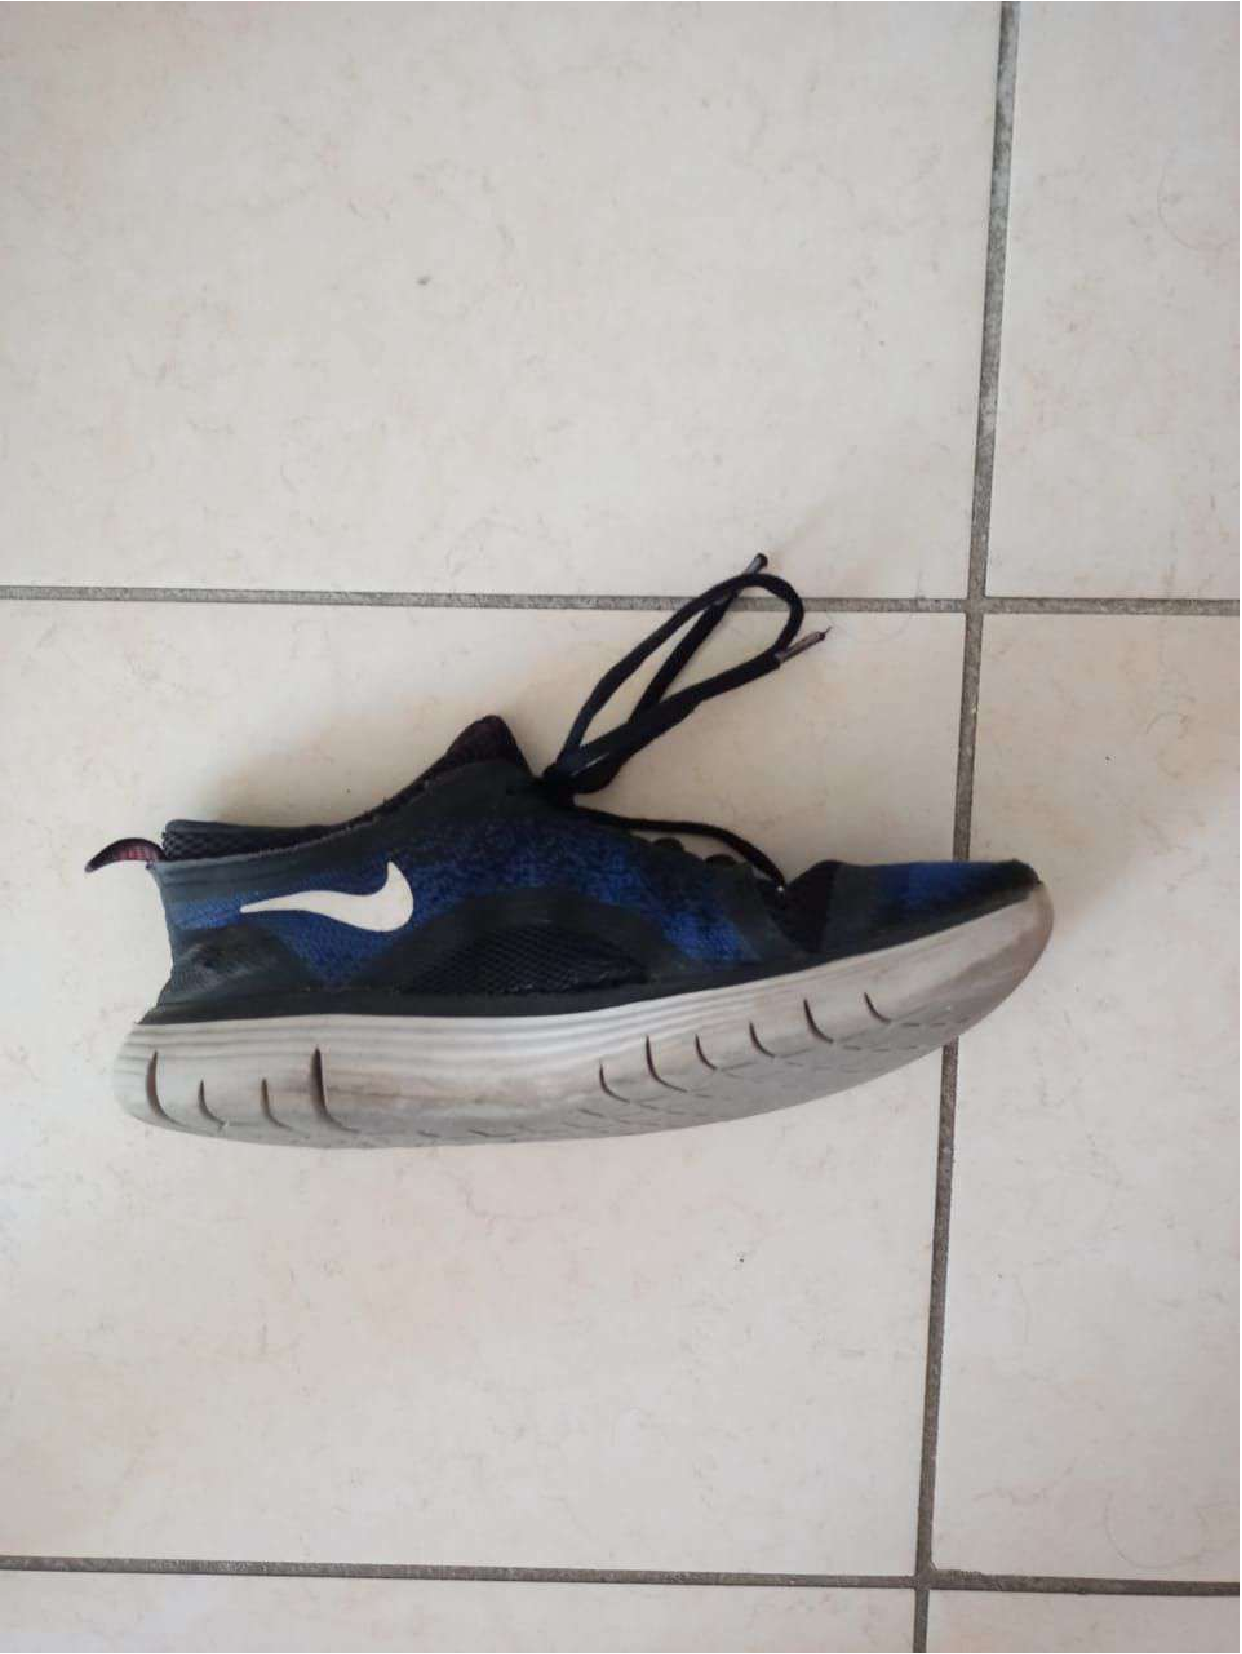
\includegraphics[scale=0.075]{fig/intro/motivation/lo_stakes/img/shoe_current.pdf}};
                \node[] at (3, 0) (out) {\emph{Nike}\\\emph{Sneakers}};
                %% Tags
                \node[] at (-3, 1.25) (intxt) {$x$};
                \node[] at (0, 1) (bboxtxt) {$f$};
                \node[] at (3, 1.1) (pred) {$y$};
                %% Arrows
                \draw[->] (in) -- (blackbox);
                \draw[->] (blackbox) -- (out);

        \end{tikzpicture}    
    \end{center}
    \pause
    \vspace{20pt}
    \begin{center}
        \textbf{We want to \emph{know why} $f(x)\rightarrow y$}
    \end{center}
    
\end{frame}
%--------------------------------------------------------------------------------------------------
\begin{frame}[t]
    \frametitle{Fitting it all together}
    \begin{center}
        \scalebox{.6}{
    %% Definitions
    \def\aicirc{(0,0) circle (3.75cm)}
    \def\mlcirc{(0.8838834764831843cm, -0.8838834764831843cm) circle (2.5cm)}
    \def\dlcirc{(1.7677669529663687, -1.7677669529663687) circle (1.25cm)}
    \def\cvcirc{(-0.8838834764831843, -0.8838834764831843) circle (2.5cm)}
    \def\nlpcirc{(0.8838834764831843, 0.8838834764831843) circle (2.5cm)}
    \def\xaicirc{(-2, -3) circle (3.75)}
    \begin{tikzpicture}
        \begin{scope}
            %% Anchors
            \filldraw[color=blue, fill=blue!5, opacity=0.5] \aicirc;
            \filldraw[color=purple, fill=purple!5, opacity=0.5] \mlcirc;
            \filldraw[color=green, fill=green!5, opacity=0.5] \dlcirc;
            \filldraw[color=red, fill=red!5, opacity=0.5] \cvcirc;
            \filldraw[color=cyan, fill=cyan!5, opacity=0.5] \nlpcirc;
            %% Text Nodes
            \node[] at (0, 4) (aitxt) {AI};
            \node[] at (0.8838834764831843, 1.8661165235168156) (mltxt) {ML};
            \node[] at (0.8838834764831843, 3.6338834764831844) (nlptxt) {NLP};
            \node[] at (-0.8838834764831843, 1.8661165235168156) (cvtxt) {CV};
            \node[] at (1.7677669529663687, -0.26776695296636865) (dltxt) {DL};    
            \pause
            \filldraw[color=orange, fill=orange!5, opacity=0.5] \xaicirc;
            \node[] at (-2, -7) (xaitxt) {xAI};
            \pause
            %% Intersection node
            \begin{scope}
                \clip \dlcirc;
                \clip \nlpcirc;
                \fill[red] \xaicirc;
            \end{scope}
            \node[] at (1, -1.25) (empt_1) {};
            \node[] at (5, -1.25) (exp) {This study!};
            \draw[->] (empt_1.center) -- node{} (exp.west);
        \end{scope}
\end{tikzpicture} 
}
    \end{center}
\end{frame}